\documentclass[11pt]{article}

\usepackage{geometry}
\usepackage{subcaption} 
\geometry{letterpaper}

\usepackage{doc}
\usepackage{cite}
\usepackage[margin=1cm]{caption}

\usepackage{url}

\usepackage{graphicx}
\usepackage{epstopdf}
\DeclareGraphicsRule{.tif}{png}{.png}{`convert #1 `dirname #1`/`basename #1 .tif`.png}

\title{Dream Design}
\author{Trixie Roque}
\date{11/24/2015}

\begin{document}
\maketitle

\begin{abstract}
The purpose of this paper is to design a new user interface for the Instagram application by integrating timeline options similar to the ones employed by Facebook, as well as allowing the users more freedom in editing their posts. Implementing these features would require integrating other APIs, such as Google Maps, for its ability to create a travel history for the user, and Snapchat, for its ability to grant users the option to doodle on their captured photos. The goal of the interface is to present the user with the power to map out a story based on their travel destinations and posts. The five usability metrics that are, therefore, involved in the creation of this design idea are learnability, efficiency, and satisfaction.
\end{abstract}

\pagebreak
\tableofcontents

\pagebreak

\section{Introduction}
\label{Introduction}
    \indent Social media applications have become a common tool in our society, especially to millennials. The ability to connect with both friends and strangers alike through the submission of "posts" onto the internet has become so widespread that it is rare to find a person that do not possess at least one social media account. Some people can even say that their hobbies involve sifting through countless blogs, tweets, videos, etc. of internet celebrities. Because of the easy access that social media applications provide us to peek through the various adventures in other people's lives, we have become incredibly immersed in them. However, even with the continuous appearance of various applications that aim to grab our everyday attention, design flaws can still exist. \\
     \indent Today's social media posts often involve clever quips, funny memes, or embarrassingly hilarious gifs or videos. 
\\
    \indent Therefore, in order to address the issues with respect to the interface design of Instagram.

\pagebreak

\section{System Description}
\label{System Description}
Although there is a desktop client for Instagram, the main focus of this paper is to address the designs in the mobile application. 

\pagebreak

\section{Top-Level Design}
\label{Top-Level Design}
The design would incorporate the Google Maps API and the Instagram API into a conglomeration that allows for posts, as well as 
The application will employ Snapchat's feature that allows the user to draw on the images. Currently, Instagram only allows various filters other lighting adjustments
\begin{figure}[ht]
\centering
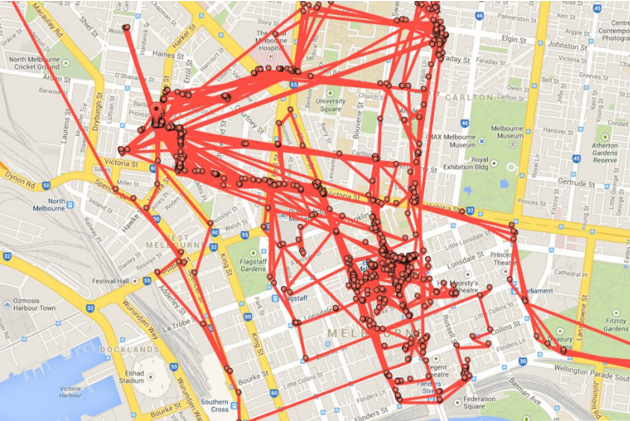
\includegraphics[width=5in]{images/google_maps_tracking.png}
\caption{Google Maps tracks users' travel history}
\label{google_tracking}
\end{figure}

\begin{figure}[ht]
\centering
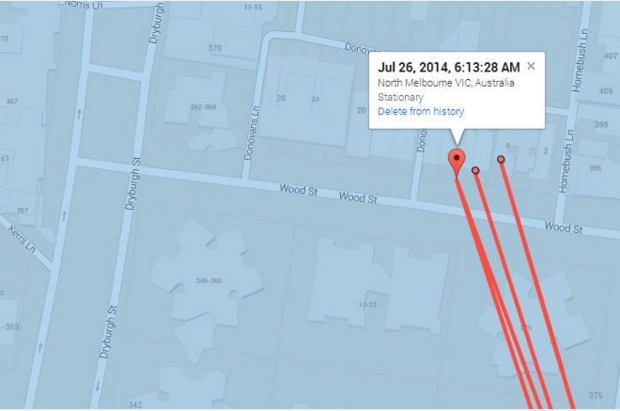
\includegraphics[width=5in]{images/google_maps_tracking_with_info.png}
\caption{The new interface would give the options to view information about the event or delete it.}
\label{google_tracking}
\end{figure}

\begin{figure}
\centering
\begin{subfigure}[b]{.5\textwidth}
    \centering
    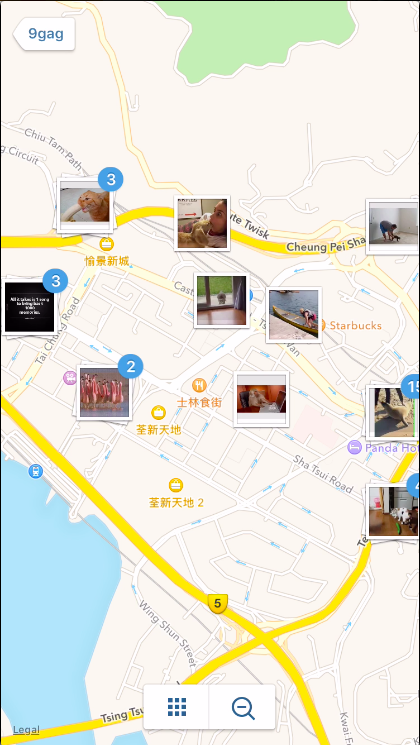
\includegraphics[height=\textwidth]{images/maps_with_pictures.png}
    \caption{Instagram already allows users to group pictures based on where they were taken.}
    \label{instagram_pictures}
\end{subfigure}%
~~~~~~~
\begin{subfigure}[b]{.5\textwidth}
    \centering
    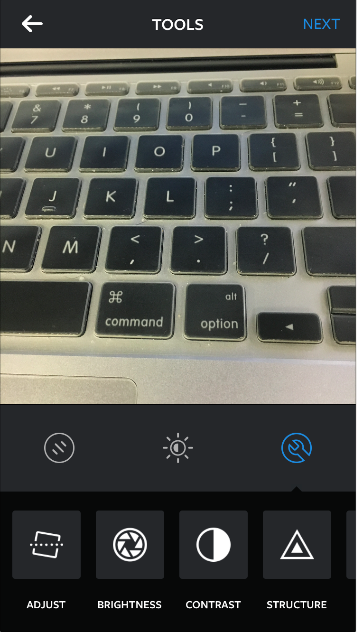
\includegraphics[height=\textwidth]{images/instagram_tools.png}
    \caption{Some tools that exist in Instagram's interface include brightness adjustments.}
    \label{tools}
    \end{subfigure}
\caption{Original features in the Instagram interface}
\end{figure}

\begin{figure}[ht]
\centering
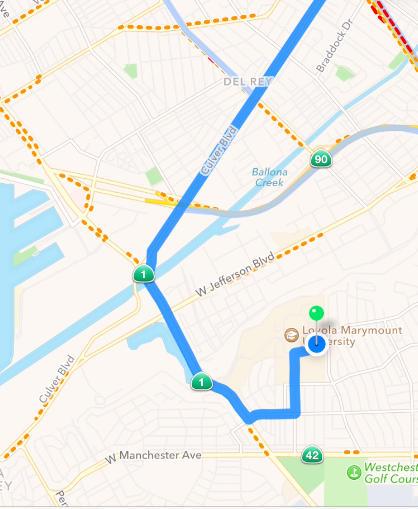
\includegraphics[width=3in]{images/gps.png}
\caption{Google Maps tracks users' travel history.}
\label{travel_history}
\end{figure}

\begin{figure}[ht]
\centering
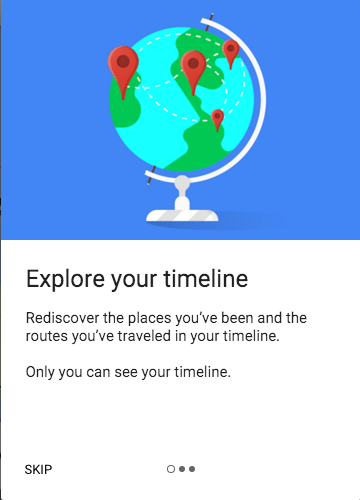
\includegraphics[width=3in]{images/view_your_timeline_prompt.png}
\caption{The new design would allow users to view where they have been, according to their posts' location.}
\label{view_timeline}
\end{figure}

\begin{figure}[ht]
\centering
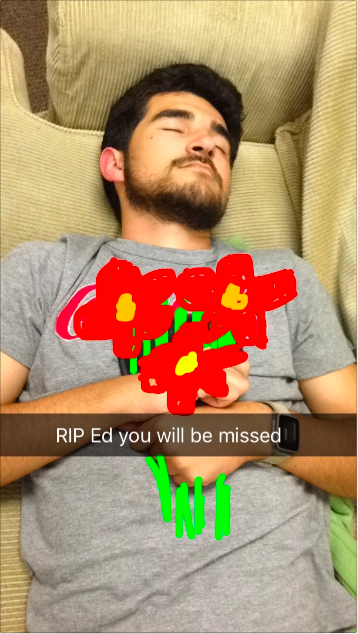
\includegraphics[height=4in]{images/rip_ed.png}
\caption{An example of doodling on a picture. The flowers were hand-drawn directly on the picture.}
\label{ed}
\end{figure}

\pagebreak

\section{Usage Scenarios}
\label{Usage Scenarios}
\indent The

\pagebreak

\section{Rationale}
\indent The

\pagebreak

\section{Usability Metric ``Forecast''}
Since the new design would integrate features that other APIs present, the usability metrics would have to be discussed. If the designs are successfully implemented and tested, given enough time, money, and manpower, the strongest metrics would have to be \\
\indent Because of the added features, the number of errors would definitely increase since the user would have more options to tap a button they did not intend to select. \\
\indent However, the strongest suit of the interface, in terms of the usability metrics discussed in class, would be satisfaction and efficiency. Because the purpose of the interface is to allow the users more freedom for their posts, consumer satisfaction is a necessary metric to fulfill. Additionally, since the interface would be implemented into a social media application, if it becomes widely used, then an expert user can easily navigate through the application's optional features.

\clearpage

\bibliographystyle{plain}
\end{document}

\end{document}